\section{Theory}

%Explain trilateration
\subsection{Trilateration}
Trilateration makes use of Equation \ref{eq_drt} to calculate the distances between the transceivers. 
\begin{equation} \label{eq_drt}
Distance = Rate \times Time
\end{equation}
Since radio signals travel with the speed of light, which is a known constant measured at exactly 299 792 458 metres per second 
\cite{young_university_2004,uzan_natural_2010}, the distance between a transmitter and a receiver can be calculated after measuring the time it takes for a radio signal to arrive at the receiver, called Time of Arrival (ToA). 

\subsubsection{Application in 2-D} \label{Trilateration2D}
In order to more easily grasp how trilateration works in theory, the application is first described for a 2-D environment.

Knowing only the distance, $D$, between a transmitter, $T$, and a receiver it is implied that the receiver is situated somewhere on the perimeter of the circle illustrated in Figure \ref{fig_circle}.
\begin{figure}[H] 
  \centering
      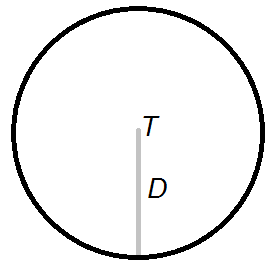
\includegraphics[height=0.25\textwidth]{img/Circle}
  \caption{An illustration of the circle with the radius given by the distance $D$ and the transmitter $T$ at its center.}
  \label{fig_circle}
\end{figure}

By measuring the distance from the receiver to another transmitter an additional circle can be calculated. Since the receiver must be situated on the perimeters of both circles it has to be located either at $A$ or $B$ as shown in Figure \ref{fig_2circles}.

\begin{figure}[H] 
  \centering
      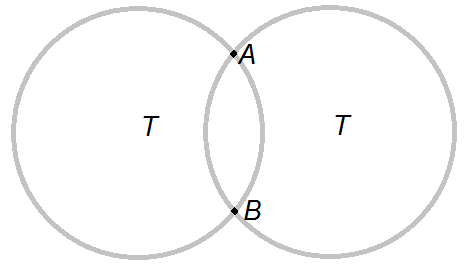
\includegraphics[height=0.25\textwidth]{img/2Circles}
  \caption{An illustration of two transmitters and their corresponding circles with intersections at $A$ and $B$ highlighted.}
  \label{fig_2circles}
\end{figure}

Repeating the previous step of measuring the distance to yet another transmitter it can be determined at which of the possible locations the receiver is situated since the three yielded circles all intersect in exactly one point as shown in Figure \ref{fig_3circles}.

\begin{figure}[H] 
  \centering
      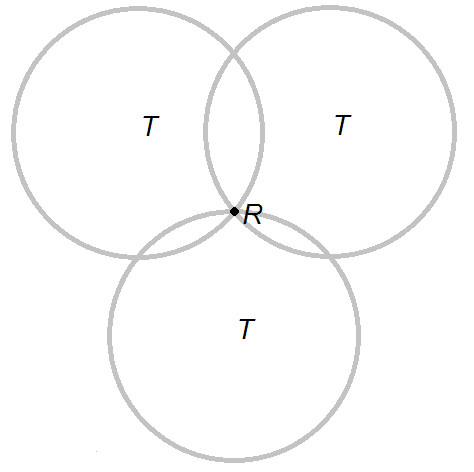
\includegraphics[height=0.45\textwidth]{img/3Circles}
  \caption{An illustration of three transmitters and the receiver shown in their intersection}
  \label{fig_3circles}
\end{figure}

\subsubsection{Application in 3-D}
Expanding the application the a 3-D environment increases the complexity as knowing only the distance between the receiver and one transmitter yields possible locations for the receiver on the peripheral of a sphere as shown in Figure \ref{fig_sphere}.
\begin{figure}[H] 
  \centering
      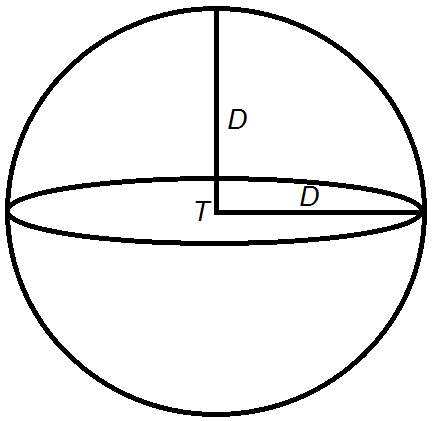
\includegraphics[height=0.25\textwidth]{img/Sphere}
  \caption{An illustration of the sphere with the radius given by the distance $D$ and the transmitter $T$ at its center.}
  \label{fig_sphere}
\end{figure}

By measuring the distance from the receiver to another transmitter an additional sphere can be calculated. Since the receiver must be situated on the peripheral of both spheres it has to be located somewhere on peripheral of the circle formed by the intersection of the two spheres as shown in Figure \ref{fig_2spheres}.

\begin{figure}[H] 
  \centering
      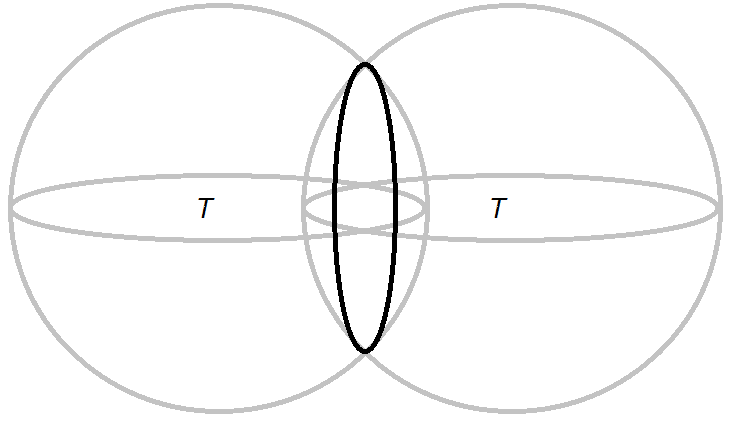
\includegraphics[height=0.25\textwidth]{img/2Spheres}
  \caption{An illustration of the two spheres and their intersection highlighted as a black circle.}
  \label{fig_2spheres}
\end{figure}

Having limited the possible locations of the receiver down to a circle, measuring the distance between the receiver and additional transmitters will decrease the possible locations in the same way as described in the 2-D environment at Section \ref{Trilateration2D}. That is, using a third transmitter limits the possible location of the receiver to two points. Sometimes it is enough to have two possible locations as the design of the positioning system may allow to rule out one of the points, that is the case with GPS where one of the points will lie in space and one will lie on the surface of Earth which has known location.

%Explain ToA?

\subsection{Two-way ranging}
As mentioned earlier trilateration depends on ToA in order to calculate the distance between a transmitter and the receiver. 
\begin{equation} \label{eq_toa}
T = T_R - T_T
\end{equation}
Calculating the ToA could be done simply using 
Equation \ref{eq_toa} as described above where T denotes the ToA, $T_T$ denotes the time when the transmitter sent the signal and $T_R$ denotes the time when the receiver received the signal. However, this method requires the transmitter and receiver to have very well-synchronized clocks since even a relatively small difference in time would result in quite a big difference in distance since it is multiplied with the speed of light.

Another method of calculating the ToA called Two-Way Ranging (TWR) eliminates the need of synchronization uses two transceivers, that is devices that serves both as transmitters and receivers allowing them to both send and receive signals. The device initiating the communication is called the leader and the other is called the follower.
\begin{figure}[H] 
  \centering
      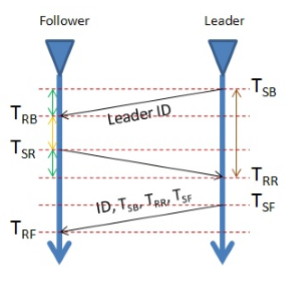
\includegraphics[height=0.5\textwidth]{img/TWR}
  \caption{Illustration of TWR}
  \label{fig_twr}
\end{figure}
Figure \ref{fig_twr} shows the scheme for TWR where $T_{SB},T_{RR}$ and $T_{SF}$ denotes the leaders send-time, receive-time and future send-time while $T_{RB},T_{SR}$ and $T_{RF}$ denotes the followers receive-time, send-time and future receive-time respectively. By subtracting the followers turn-around time from the leaders round trip time as shown in Equation \ref{eq_twr1}, the time it takes for a signal to travel from the leader to the follower and back is calculated giving twice the transmission time $T_T$, which is the same as the ToA. 
\begin{equation} \label{eq_twr1}
2T_{T} = (T_{RR} - T_{SB}) - (T_{SR} - T_{RB})
\end{equation}

After the leader receives the response from the follower it responds with another signal enabling an additional calculation of the ToA using Equation \ref{eq_twr2}.

\begin{equation} \label{eq_twr2}
2T_{T} = (T_{RF} - T_{SR}) - (T_{SF} - T_{RR})
\end{equation}

By taking the average of the two ToA calculations, resulting in Equation \ref{eq_twr3}, the final value of the ToA is calculated.

\begin{equation} \label{eq_twr3}
T_{T} = \frac{T_{RF} - T_{SF} + 2(T_{RR} - T_{SR}) + T{RB} - T_{SB}}{4}
\end{equation}
\clearpage